\documentclass[frame, english]{idamasterthesis}
%\usepackage[utf8]{inputenc}
\usepackage{amssymb}
\usepackage{amsmath}
\usepackage{amsfonts}
\usepackage{mathtools}
\usepackage{enumitem}
\usepackage{url}
\usepackage{dblfloatfix}
\usepackage{graphicx}
\usepackage[final]{pdfpages}


\author{Tomas Melin and
    Tomas Vidhall
    }

\titleenglish{Namecoin as authentication for public-key cryptography}
\titleswedish{Namecoin som autentisering för asymmetrisk kryptering}
\dateofpublication{2014-05-26}
\supervisor{Marcus Bendtsen}
\examiner{Nahid Shahmehri}
\degreesubject{Engineering}
\supportedby{SUPPORTEDBY}

\facultyexaminername{OPPONENT NAME}
\facultyexaminertitle{OPPONENT TITEL}
\facultyexamineraddress{OPPONENT ADDRESS}

\abstract{ \S\ Public-key cryptography is a subject that is very important to everyone who wants confidentiality and privacy in networks. It is important to understand how public-key cryptography systems work and what flaws they have. In the first part of this report we describe some of the most common encryption schemes and key agreements. We carefully investigate their flaws, if they are broken and what threats have dire consequences. \abstractpar \noindent We found that the biggest issue is authentication and we present current solutions to the problem. The current solutions are flawed because they rely too much on trusting different entities. It is only required that one trusted entity becomes malicious for the entire authentication system to be compromised. Because of this we propose an alternative system in the second part, Namecoin. A risk analysis in form of an attack tree is performed on the Namecoin system, where we describe how the attacks are executed and what you can do to prevent them. We present different threats against the system and we describe how dire the consequences are and the probability of their execution. Since Namecoin is an implementation of the block chain algorithm we have also explained how the block chain works in detail. \abstractpar \noindent We present why we think that Namecoin is a system that should replace the currently used certificate authority system. The certificate authority system is flawed because it is centralized and dependant on that no authority makes any mistakes. The Namecoin system does not become compromised unless more than $50 \, \%$ of the hashrate in the system is used with malicious intent. We have concluded that the biggest threats against Namecoin have such a low probability that they can be neglected. 
}

\begin{document}
\small

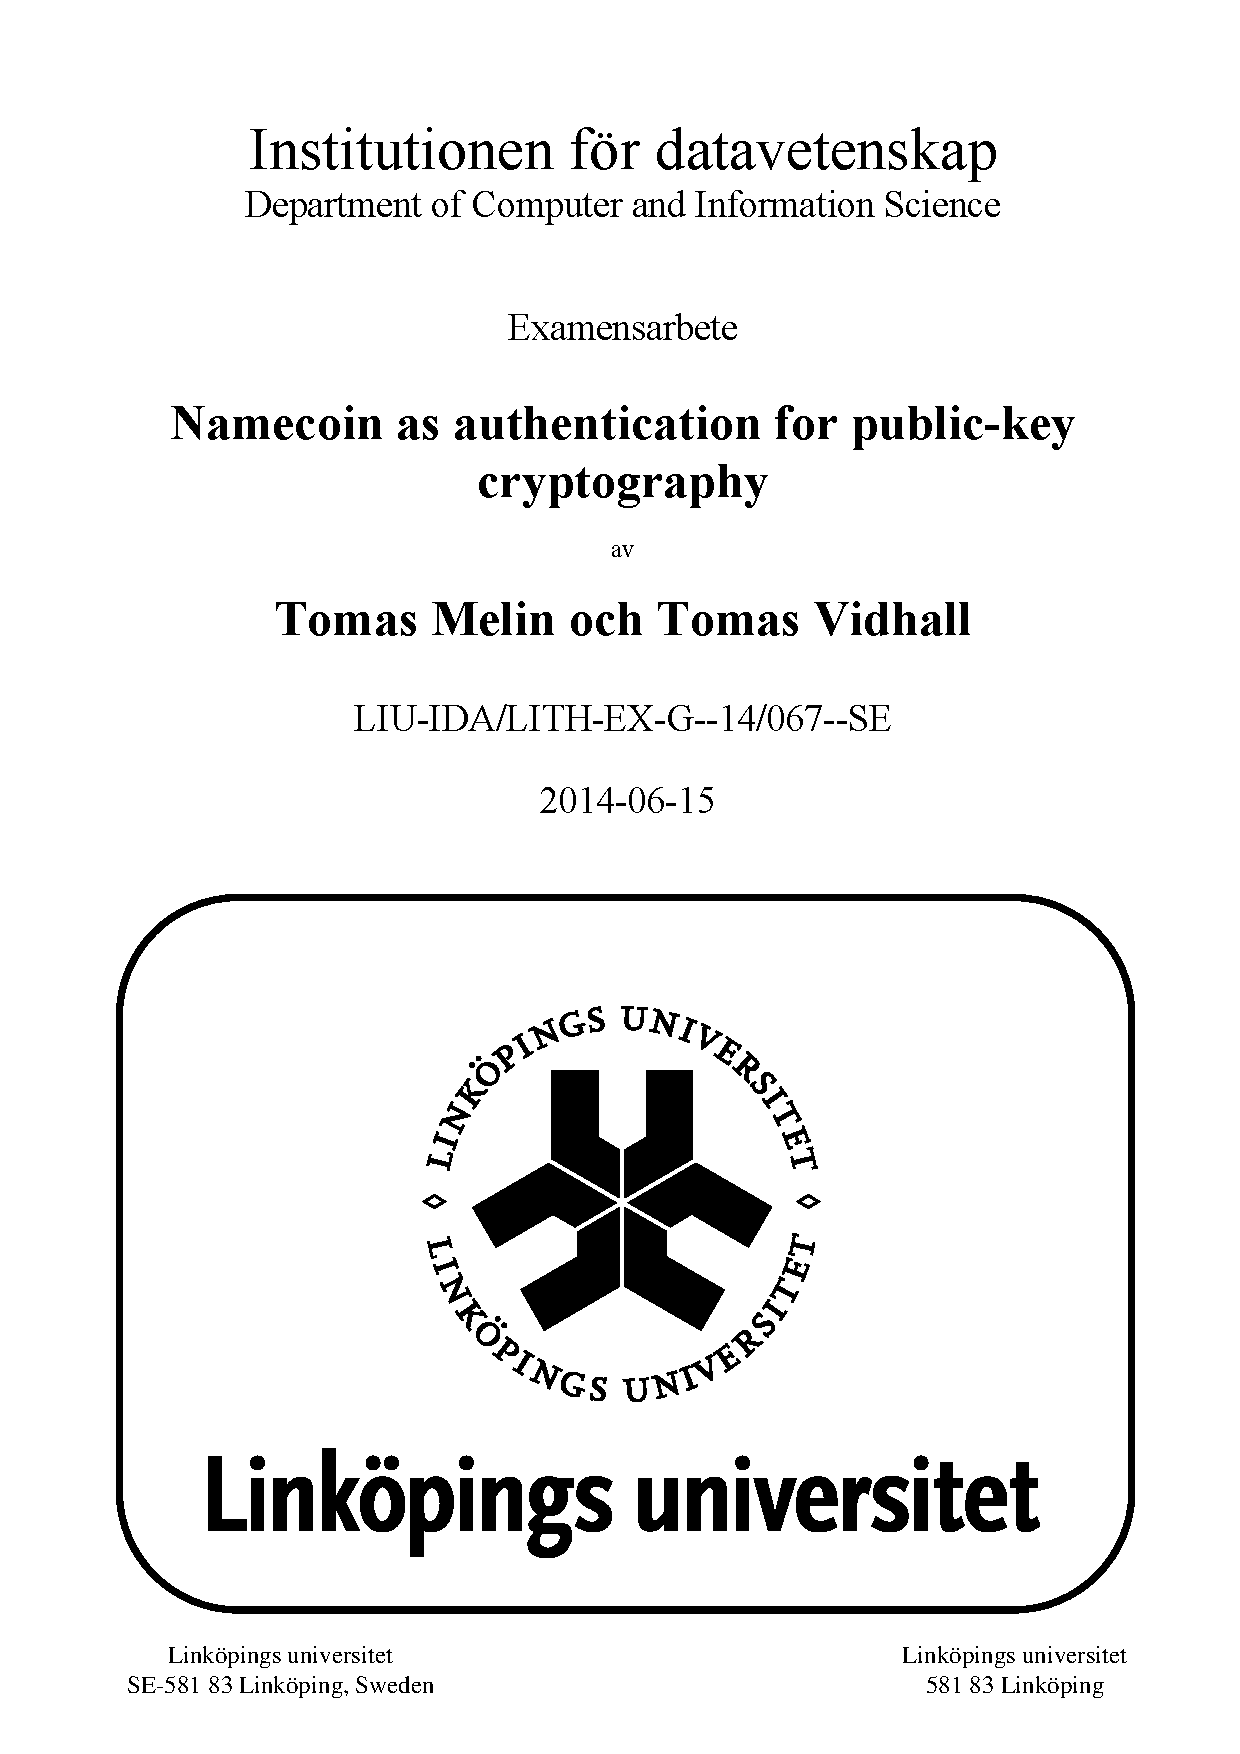
\includepdf[]{PDFs/titelsid-sv.pdf}
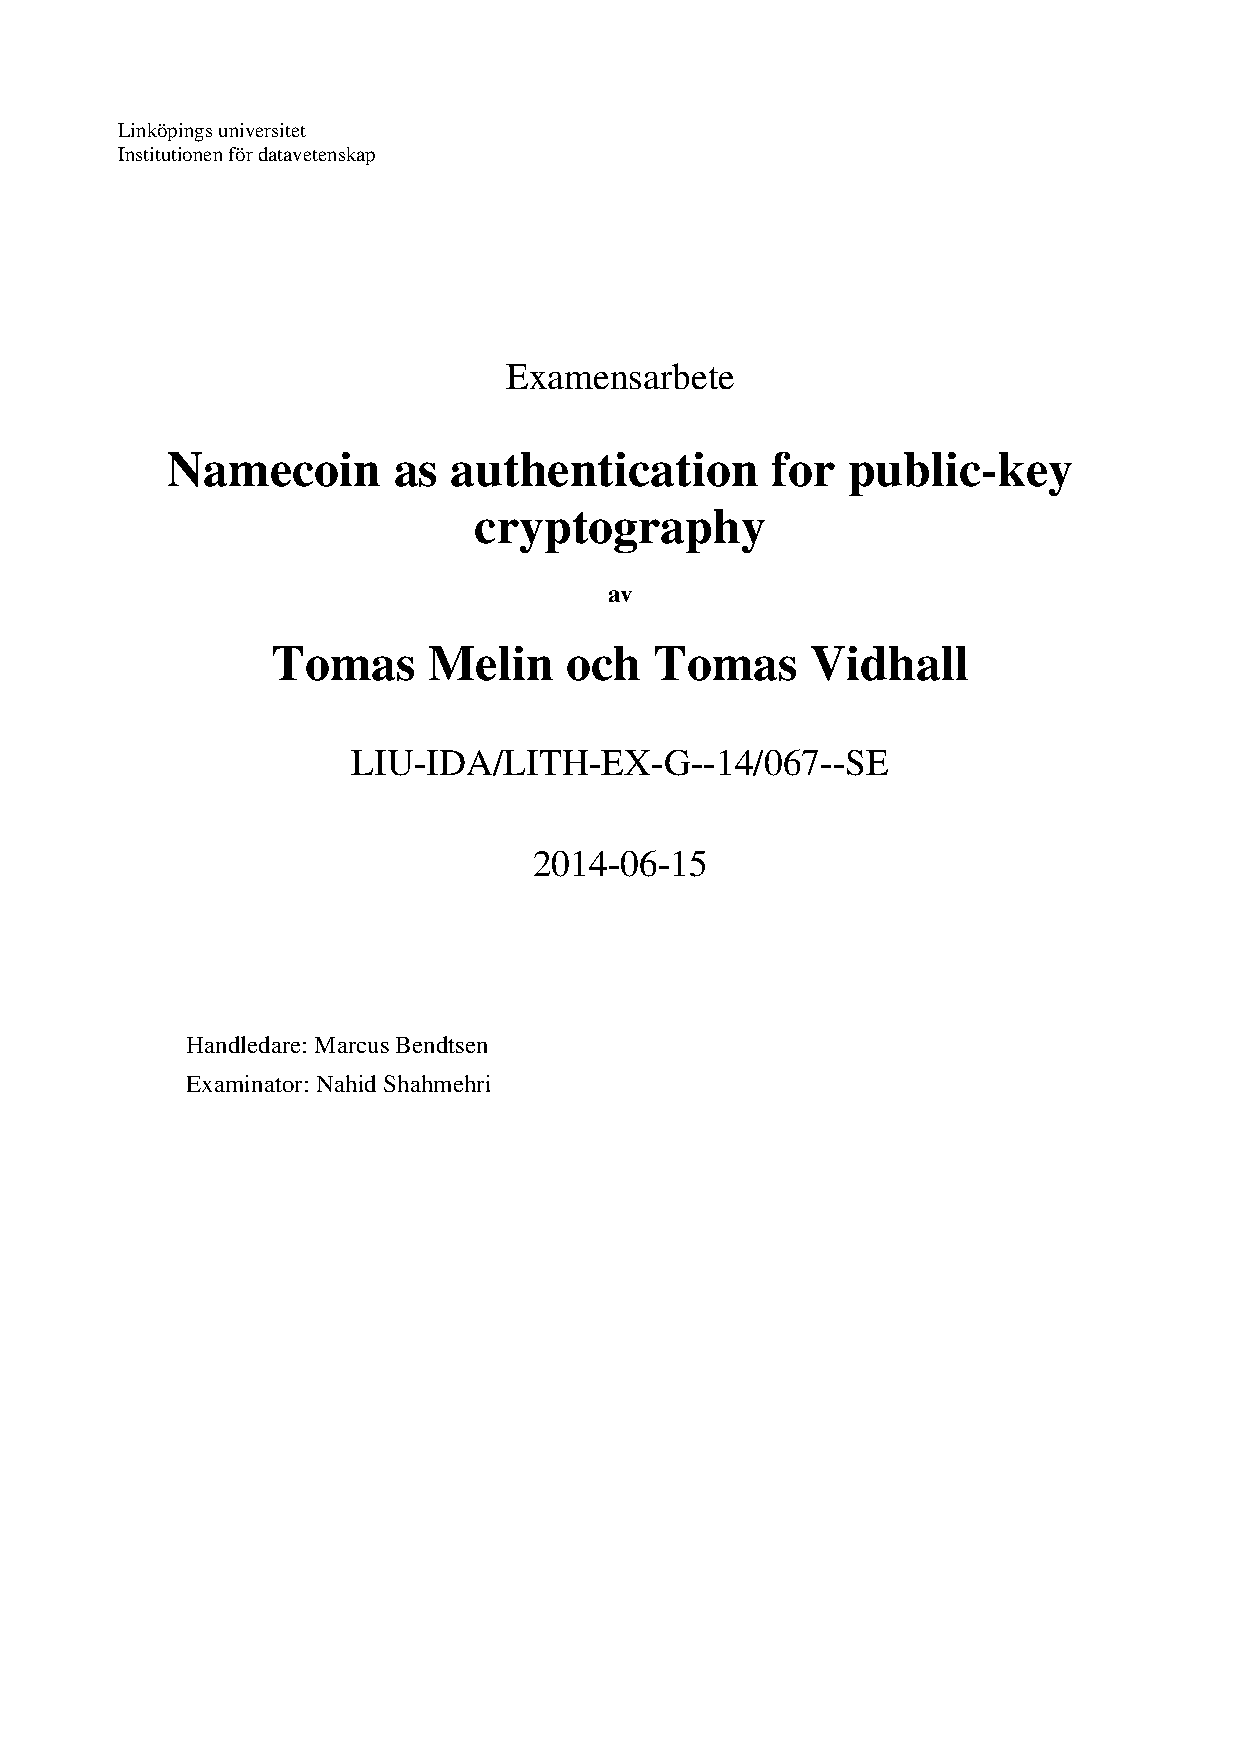
\includepdf[]{PDFs/insid-sv.pdf}

\makeintropages

\chapter{Introduction}
\chaptermark{}
Public-key cryptography is a procedure with the main objective to ensure integrity and
confidentiality. The procedure uses two keys, a public and a private key. A user has a public key that is used to encrypt messages and can be shared in any possible way. The same user also has a private key which is only known by the user. If the user receives a message that is encrypted with her public key she can decrypt it with her private key and no one else can decrypt it. \\\\
This can be further explained using mathematical notations. An entity has a public key $e$ and a corresponding private key $d$. For a system to be secure, it has to be theoretically infeasible to compute $d$, given $e$. The public key defines an encryption transformation $E_e$ and the private key defines the associated decryption transformation $D_d$. This means that if an entity $B$ wants to send a message to $A$, it has to retrieve a copy of $A$'s public key $e$ and use $E_e$ to obtain the cipher text $c=E_e(m)$, where $m$ is the message in plain text, and send $c$ to $A$. Once $A$ has received the cipher text $c$, $A$ uses $D_d$ with the private key $d$ to decrypt the cipher text into the original message in plain text $m=D_d(c)$ \cite{handcrypt}.

\section{Motivation and purpose}
The concept behind private and public keys is very fascinating to us and we also know that it is very hard to decrypt data which have been encrypted with a public key. This makes us motivated to study public-key encryption more carefully and investigate the subject thoroughly. We plan to find the advantages and the disadvantages of using public-key encryption and how it is possible to take advantage of the implementation flaws.

\subsection{Questions of interest}
The work is divided into two parts, the first which contains a historical review of public-key encryption that highlights the developments and the known vulnerabilities of these systems. This first part aims to answer the following questions:

\begin{itemize}
    \item How does public-key cryptography work? 
    \item What attacks are public-key cryptography vulnerable to today? 
\end{itemize}

\noindent
The second part is an in-depth look at an alternative way for authentication using public-key encryption that could solve some of the known issues.

\begin{itemize}
    \item Is it possible to reduce the number of threats against public-key cryptography using authentication?
    \item How can we authenticate public keys in a secure way?
\end{itemize}
    
\chapter{Historical review}
\chaptermark{}
In this chapter we will give a historical review of public-key encryption and its flaws. The following sections contains material about public-key encryption schemes, key agreements and authentication. These topics are important to understand due to the proposed solution in the second part of this report. 

\section{Public-key encryption schemes}
The next section will present various public-key encryption schemes. The schemes which we will discuss represents a large portion of the major public-key encryption schemes which have had a historical impact. The procedure which these encryption schemes use to generate their key is different from scheme to scheme, however in this report we will only show how RSA generates the private and public key. We chose to only describe RSA because it is the most used public-key encryption scheme today. We will also describe the Diffie-Hellman key exchange because it is the most prominent key-exchange, using techniques similar to public-key encryption.\\\\
\noindent
The timeline in Figure~\ref{usagetimeline} contains the encryption schemes and public key exchanges which we will mention in this report. Both the McEliece  and Merkle-Hellman knapsack public-key encryption schemes have been broken. 

\begin{figure}[h!]      %   PIC:USAGETIMELINE 
    \centering
    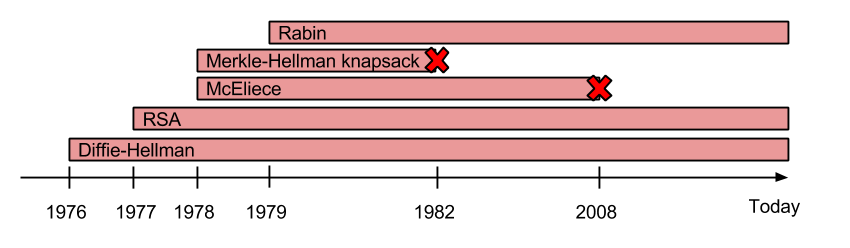
\includegraphics[width=80mm]{Pics/timeLineUsage.png}
    \caption{A timeline showing when these public-key encryption schemes and key agreements were published and broken. }
    \label{usagetimeline}
\end{figure}

%   RSA
\subsection{RSA public-key encryption}
RSA is short for R. Rivest, A. Shamir, and L. Adleman and is the most widely used public-key cryptographic system \cite{handcrypt}. RSA's security is based on the intractability of the integer factorization problem. That is, given a positive integer $n$, your task is to find its prime factorization.

\pagebreak

\noindent The key generation for RSA consists of five steps. Each entity is required to have a RSA public key and a corresponding private key. 
    
\begin{enumerate} % RSA KEY GENERATION
    \item Generate two large random (and distinct) primes $p$ and $q$, each roughly the same size. 
    \item Compute $n=pq$ and $\phi = (p-1)(q-1)$
    \item Select a random integer $e$, $1 < e < \phi$, such that $gcd(e,\phi)=1$, where $gcd(x,y)$ is the greatest common divisor for $x$ and $y$. 
    \item Use the extended Euclidean algorithm to compute the unique integer $d$, $1<d<\phi$, such that $ed \equiv 1 (\bmod \phi)$
    \item The entity's public key
    is $(n,e)$ and the private key is $d$.\hfill \cite{handcrypt}
\end{enumerate}
    The algorithm for RSA public-key encryption has two phases, encryption and decryption \cite{handcrypt}.
\begin{description}
    \item[Encryption] In this case, $B$ encrypts a message $m$ for $A$, which A decrypts.
    \begin{enumerate}
        \item Obtain A's authentic public key $(n,e)$.
        \item Represent the message as an integer $m$ in the interval $[0,n-1]$.
        \item Compute $c=m^e \bmod n$, using the extended Euclidean algorithm.
        \item Send the cipher text $c$ to $A$. 
    \end{enumerate}
            
    \item[Decryption] To recover plain text $m$ from $c$, $A$ should do the following: 
    \begin{enumerate}
        \item Use the private key $d$ to recover $m=c^d \, \bmod n$. \\
    \end{enumerate}
\end{description}

\noindent
RSA has a lot of practical implementations and is used all over the Internet, but it can mostly be categorized into two main uses, digital signatures and encryption of data. Digital signatures is a way to authenticate that someone that is identified with a public key is who she says she is. Since the encryption in the RSA-algorithm is two-way, you can both encrypt with the public key and the private key. If you encrypt with the public key you can decrypt with the private key and vice versa. Because the private key is not public, only the person who knows this key can encrypt with it. If you send a message you can also sign this message through adding data encrypted with your private key. Now someone who receives this message can decrypt its data using your public key and therefore authenticate your identity. \\\\
The earliest version of RSA is from the 1970s, however, this is not the version used today. This early version of RSA is what is called the textbook version of RSA, i.e. the version that is taught but is not actually used. The difference between the textbook version and the version of RSA that is being used in the real world is that the non-textbook version uses what is called \emph{padding}. Padding involves inserting a structured randomized sum of characters into the message $m$, which is to be encrypted. This is done in order to separate two equal messages from having similar cipher texts. If they did have similar ciphertexts an attacker could easily see patterns in the ciphertexts. From these patterns you can draw conclusions about the non-encrypted message. With padding this is avoided and every message is seemingly random \cite{handcrypt}.

\pagebreak

\noindent
Well known implementations of RSA include digital signatures in certificates for Secure Socket Layer/Transport Layer Security (SSL/TLS) and authentication in Secure Shell (SSH). In SSL/TLS, RSA is used for digitally signing certificates. You verify the identity of an entity by checking that the signature is valid. If it is valid you can trust that the public key in the certificate really is the entity's public key \cite{ssl}.\\\\
In SSH it is mostly used as a way to confirm your identity. SSH uses a list of trusted public keys which are allowed to connect and if your key is on this list you may connect. In this manner RSA is used as a sort of doorman \cite{ssh}.\\\\
Lately there has been a lot of reports about RSA Security LLC having included a backdoor in the RSA-algorithm, for the American security organization NSA. Reportedly they got paid \$10 million to implement a security flaw in the randomization algorithm which NSA could easily take advantage of. The problem with this is that they compromised the security of everything that is built on RSA when they knowingly implemented this backdoor. This can make users have trust issues with RSA and can make people look for other standards of public-key cryptography \cite{nsabackdoor}.\\\\
Recently there has been progress in using a special sort of side channel attack to break something as secure as RSA with a 4096-bit key length. This special attack uses the sounds of the processing unit during decryption of secret data \cite{rsasound}. When the computer is decrypting it will produce sounds between 10 and 150 KHz and if you record these you have all the data you need. Now the hard part is to actually differentiate the private key sounds from the rest of the data. Since this is non-random it is easily doable with a sufficient amount of data. Once you have decoded the private key the system is compromised. The dangers of this attack is that they could actually decrypt data just by having a cellphone approximately 30 cm away from your computer. Because attacks like these are possible, it is not always enough to only protect your data with encryption. The actual physical representation of the data, for example a hard drive, also has to be secured.

%   MERKLE-HELLMAN KNAPSACK
%   TODO: FÄRRE STEG, ENDAST KRITISKA STEG
%   TA FRAM DET STEG SOM GÖR ATT DEN GÅR ATT KNÄCKA
%   Knäckt av Shamir 1984 % 1982? Jag hittade 1982 :O TODO
\subsection{Merkle-Hellman knapsack encryption}
Merkle-Hellman knapsack encryption is the first concrete realization of a public-key cryptographic system \cite{handcrypt}. It is based on the mathematical problem called the \textit{superincreasing subset sum problem}. It differs from RSA through the encryption being only one-way. The public key is only used for encryption and the private key is only used for decryption. You can not get a message encrypted with the private key and decrypt it using the public key and therefore it can not be used for cryptographic signing \cite{handcrypt}. \\\\
Shamir has described an algorithm which is able to break the Merkle-Hellman knapsack encryption in polynomial time, hence it is broken and can not be used in a secure way \cite{merklebroken}. The consequences of this breaking was not great due to the fact that it had only existed for four years and thus, had not been implemented on a large scale.  

%   MCELIECE    
\subsection{McEliece public-key encryption}
The McEliece public-key encryption scheme is based on the difficulty of decoding a general linear code, i.e. an error correcting code where any linear combination of code words is also a codeword \cite{code}. 
The idea behind this scheme is to first select a particular code for which an efficient decoding algorithm is known, and then to disguise the code as a general linear code. Due to the fact that the procedure of decoding an arbitrary linear code is NP-hard, a description of the original code can serve as the private key and a description of the transformed code serves as the public key \cite{handcrypt}.\\\\
In 2008 \cite{attackdefence,analysmce} an attack was described which could break the McEliece public-key encryption in 1400 days by a single computer (2.4GHz Core 2 Quad CPU) or in only 7 days by a cluster of 200 CPUs, where no communication was needed between the computers. The approach of the attack was based on Stern's attack of finding low-weight\footnote{A codeword's weight is the number of elements that are nonzero.} codewords in a slightly larger code. The event of breaking McEliece have not had severe consequences, since it can still be used if the keys are increased in size. This does however increase the time it takes to encrypt and decrypt messages and this has prevented it from being able to compete with other encryption schemes \cite{handcrypt}.  

\subsection{Rabin public-key encryption} 
Rabin is the first example of a provably secure public-key encryption scheme \cite{rabinorig}. Many cryptographic systems, for example RSA, are believed to be as hard to break as the mathematical problems they build on, but few algorithms is provably secure. Rabin is one of those which has been proven to be as secure as the related mathematical problem, the integer factorization problem. Rabin works just as RSA except for differences in the key-generation. \\\\
The same property that provides Rabin to be provable secure, also implies a disambiguation which introduces additional computational costs. This disambiguation is what has prevented the Rabin cryptographic system from finding widespread practical use \cite{handcrypt}.

%   DIFFIE-HELLMAN
\subsection{Diffie-Hellman key exchange}
Although not strictly a public-private key scheme, Diffie-Hellman utilises a public-private key algorithm to facilitate symmetrical encryption.
A key agreement is an initialization process that enables symmetric encryption. It is a way of agreeing to a mutual secret key on an open channel where only the involved parties can determine the secret key. We will be discussing the Diffie-Hellman key exchange because it is one of the most used key agreements. The security is based on the intractability of the Diffie-Hellman problem and the related problem of computing discrete logarithms.

\pagebreak
\noindent
The Diffie-Hellman key exchange is a key agreement which makes secure symmetric encryption possible. This is done to ensure that the communication over a insecure channel is not compromised by a third party. \\\\
$A$ and $B$ are communicating over an open channel.
The procedure is performed as follows: \cite{handcrypt}
\begin{enumerate}
    \item One-time setup. An appropriate prime $p$ and generator $\alpha$ of \\ $\mathbb{Z}^{*}_{p} \; (2 \leq \alpha \leq p - 2)$ are selected and published.
    \item Protocol messages (used in step 3).
    
    \begin{equation}    %   (2.1)
        A \rightarrow B : \alpha^x \bmod p 
    \end{equation}
    \begin{equation}    %   (2.2)
        B \leftarrow A : \alpha^y \bmod p
    \end{equation}
    
    \item Protocol actions. Perform the following steps each time a shared key is required. 
    \begin{enumerate}
        \item $A$ chooses a random secret $x$, where $1 \leq x \leq p - 2$, and sends $B$ message (2.1).
        \item $B$ chooses a random secret $y$, where $1 \leq y \leq p - 2$, and sends $A$ message (2.2).
        \item $B$ receives $\alpha^x$ and computes the shared key as $K = (\alpha^x)^y \bmod p$.
        \item $A$ receives $\alpha^y$ and computes the shared key as $K = (\alpha^y)^x \bmod p$. \\
    \end{enumerate}
\end{enumerate}

\noindent
Diffie-Hellman is widely used in among other things SSL/TLS, SSH and Internet Key Exchange (IKE). In all applications it is used to agree on a secret symmetric key for further communication. The big problem with this is that first you need to authenticate the user you are communicating with. For example in SSL/TLS the authentication happens through certificates and RSA as mentioned earlier (in section 2.1.2). The most common attack used against a key agreement is the later mentioned man-in-the-middle attack (see section 2.5.1). If you do not properly authenticate whoever you want to communicate with, you could be victim to the attack and there would be no way for anyone involved to notice that you were being attacked. Because of this we can see the importance of proper authentication \cite{ssl,ssh,ike-rfc,kerber-rfc}.

\section{The mathematical problem}
Both Diffie-Hellman and RSA rely on related mathematical problems to ensure security. Advances in solving the discrete logarithm problem usually leads to advances in the integer factorization problem, which means that if one is solved, the other is also compromised. There has been little progress in finding a polynomial time algorithm for solving these problems since the 1980s. Since February 2013 there has been rapid progress in this field, mostly due to a man named Antoine Joux from France. He has started making real progress in solving these problems and therefore future security researchers are looking for new mathematical problems \cite{math}.

\section{Authentication}
Public-key encryption may be appealing in theory because of its extensive mathematical properties. There are however some issues and one of the most prominent is authentication. If someone sends you their public key, how do you know that they are who they claim they are? If you do not properly authenticate someone you want to communicate with, the encryption is pointless because you do not know who is getting the information. This implies that there is a problem with the implementation of the solution, rather than a mathematical fault. In the following subsections we will discuss some current solutions to the authentication problem. We will frame the discussion with the man-in-the-middle attack, which shows how an attack can take advantage of authentication weaknesses.

\subsection{Man-in-the-middle attack}
A man-in-the-middle attack is an attack which takes advantage of the problem with authentication.  An example would be that you are requesting the public key of Google with a message to their address. The attacker catches the message and sends back her public key instead of Google's. Now you will of course assume that you have Google's public key and can send encrypted messages to them. The attacker will take your packets, read them, and send them to Google. When Google responds the attacker will read the response and forward it to you. She can do all of this without leaving any traces and neither you nor Google will know that she could read your "encrypted" information. To send secure encrypted information we need some sort of authentication to prove that you are who you say you are \cite{maninthemiddle}. \\\\
In Figure~\ref{fig:mitm} it is illustrated how a man-in-the-middle attack can be performed. The blue arrow represents the path that the client and the server expects the traffic to travel. The red arrows represent the actual path, via the attacker, which the traffic travels. 

\begin{figure}[h!]      %   PIC: MITM
    \centering
    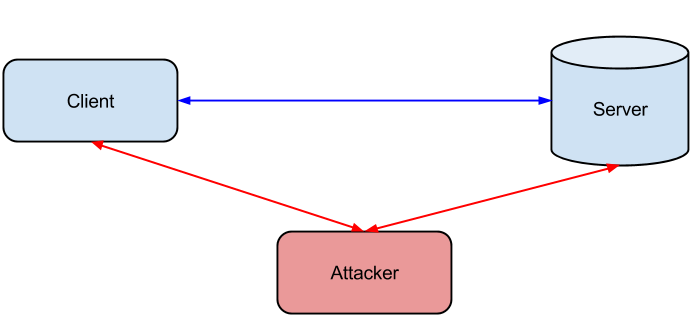
\includegraphics[width = 75mm]{Pics/mitm.png}
    \caption{A figure illustrating how a man-in-the-middle attack works.}
    \label{fig:mitm}
\end{figure}

\pagebreak

\subsection{Certificates and certificate authorities}
In order to connect a resource to a person or an organization, e.g. to authenticate that a website is who it say it is, the most used solution is to use certificates. A certificate is proof that the public key $P$ really is the public key of the entity $E$ that you are trying to contact. A public-key certificate normally contains a number of fields, such as: 
\begin{itemize}[noitemsep]
    \item Version - The version of the certificate.
    \item Issuer - The certificate authority who issued the certificate.
    \item Serial number - A unique identifier for the issuer.
    \item Subject - The entity $E$ for whom the certificate was created. 
    \item Subject public key - The public key of the entity $E$.
    \item Signature value - A signature that can be verified with the public key of the issuer (encrypted hash).
    \item The signature algorithm - The algorithm that was used to create the signature.
    \item Validity - The time frame in which the certificate is valid. 
\end{itemize}

\noindent
The certificate authenticates the subject's public key and that the subject is who she says she is. To authenticate this you need to decrypt the signature value with the public key of the issuer. Now you have the hash value of the certificate and you need to verify this. Therefore you use the signature algorithm, provided in the certificate, to hash the content of the certificate.\\\\
If this value is the same as the decrypted signature value you have validated the information in the certificate and you know the subject's public key. This solution has one problem though, how do you know that the issuer's public key is correct? \\\\
The issuers of these certificates are called certificate authorities (CAs). They are companies that are "trustworthy" and therefore their public keys are already installed in software such as operating systems and browsers. Because of this, we can always use the CA's public key to verify a public key of someone who bought a certificate from the CA. Most CAs also has a certificate for all other CAs and therefore they create a chain of authentication. This way every CA verifies all certificates signed by any other CA \cite{certificate}. \\\\
The solution is flawed in the sense that the entire Internet trusts these CAs blindly. If one of these CAs starts to produce non-valid certificates everyone will still trust these, because the CA is trustworthy. Even if it is a complex and difficult process to become a verified CA we still have to put our trust in the system and actually believe that no CA will become malicious. There has been several issues with CAs and lately both a French and Dutch CA has been caught creating non-valid certificates \cite{frenchCA,dutchCA}.

\pagebreak

\noindent
Figure~\ref{fig:certauth} illustrates how the Certificate authority system works. The user first requests to connect to a website which is controlled by the server. In order to be certain that the website is controlled by the authority which it says it is, the user then runs a control with the CA. If the control gives the result that proves that the authority behind the requested website is who is given by the website, the user can be certain that she is not being eavesdropped on by some malicious authority. In Figure~\ref{fig:certauth} the blue arrow represents communication which is done in order to control whether the certificate of the requested website is valid and the purple arrow represents secure traffic between the user and the server. 

\begin{figure}[h!]      %   PIC: Certificate authorities
    \centering
    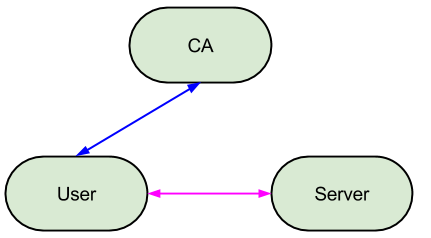
\includegraphics[width = 40mm]{Pics/CA.png}
    \caption{A figure illustrating how Certificate authorities works.}
    \label{fig:certauth}
\end{figure}

\subsection{Web of trust}
Web of trust is another solution to the problem with authentication in public-key encryption systems and is an alternative to the centralized trust model of public-key infrastructure which involve CAs. It can be thought of as a peer-to-peer network with nodes, some that you trust and some that you do not trust. The idea of the Web of trust concept is to search for another node in the network which has verified the key, i.e. confirmed that the public-key is legitimate. If you can find a trusted node, $N_1$, which verifies the public key of the node you want to verify, $N_2$, then the public key of $N_2$ is verified. \\\\
Every time that you want to verify a public key you have to be certain that you can trust every trusted node. Because of this, the system is very volatile and you have to constantly check for malicious nodes. If only one node has become malicious they can send you the wrong data and your communication may be compromised. It is also hard to use on a large scale since the nodes you trust can verify different nodes. If I do not trust $N_1$ and she is the only one that can verify $N_2$, then I can never verify $N_2$ without trusting $N_1$. The sum of this is that the Web of trust does not really solve the problem with authentication in a good enough way to be implemented on the Internet \cite{rubin}.

\pagebreak

\noindent
Figure~\ref{fig:weboftrust} shows how $A$ requests the key of $N_1$. A purple connection represents a request, a blue connection represents nodes which know the corresponding public keys and a green connection represents trusted nodes. In this case $N_3$ will send a response containing the public key of $N_1$ to $A$ and they can now communicate securely.

\begin{figure}[h!]      %   PIC: Web of trust
    \centering
    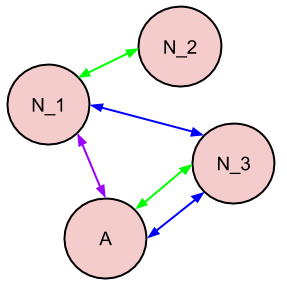
\includegraphics[width = 30mm]{Pics/weboftrust.png}
    \caption{A figure illustrating how Web of trust works.}
    \label{fig:weboftrust}
\end{figure}

\section{Summary of historical review}
The first part of this report aimed to explain how public-private key cryptography works and what attacks it is vulnerable to today. Through a historical review we have presented some common public-private schemes and their weaknesses. The mathematical properties of some of these schemes are theoretically safe, however when they have been implemented a new issue has been found, authentication. The next part of this report will look into an alternative system for solving the issue of authentication, Namecoin. A risk analysis in the form of an attack tree will also be performed on the Namecoin system. This will present the major threats and risks for this authentication system and we will compare these to the issues of the current solutions.

\chapter{Namecoin for authentication} \chaptermark{}
Due to the issues of authentication, presented in part one, we have found an alternative solution, using the Namecoin system for authentication. In this part we will present the theory behind Namecoin, the block chain and a risk analysis of the Namecoin system. A comparison will be made between the current authentication systems and the Namecoin system.

\section{Theory}
The block chain is a sort of online bulletin-board where you can not change things without having a majority of the network behind you. To make decisions based on majority agreement in a peer-to-peer network is something that can be used to authenticate users. To do this you can use the block chain algorithm. A very popular implementation of the block chain algorithm is the cryptographic currency Bitcoin \cite{bitcoin}.

\subsection{Transactions}
A transaction is some data that you want to be visible to everyone in the network. For example in the Bitcoin-implementation you want to show everyone how many and to whom you sent the Bitcoins. This data is different in every implementation and depends on the purpose of the block chain.

\subsection{The block}
A block consists of a header and a body. The header contains information about the previous block, the difficulty of creating the block, a unique address to the creator of the block, a counter and other data depending on the implementation. The body contains information about transactions that have occurred in the network and is not present in a previous block.

\subsection{The chain}
Because the previous block hash is kept in the header of every block, a block chain is created from the current block all the way to the genesis block. A block can only have one previous hash and therefore two block chains can never merge together, but they can diverge. Every time a block is created the creator broadcasts this to the rest of the network. When a new block is received the user tries to create a new one with with the recieved one in the header. The longest chain is always the one that is considered the real chain and if two blocks are found at the same time you will end up with two forks of the block-chain. Depending on which one of these grows the fastest it will be considered to be the main branch of the block chain. Meanwhile the chain that did not grow as fast will be left and all transactions in these blocks will be considered non-existent by the main branch. 

\begin{figure}[h!]      %   PIC: Blockkedjan
    \centering
    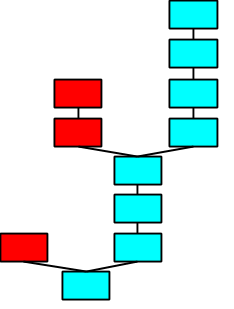
\includegraphics[width = 25mm]{Pics/blockkedjan.png}
    \caption{A figure showing how a part of the block chain can look. Red blocks are not part of the longest chain and cyan blocks represent the main branch. }
    \label{fig:blockchain}
\end{figure}

\subsection{Creating a block}
To create a block you create a new block header including a hash of the previous block header, a number that describes the difficulty $d$ that the network has agreed upon, a counter $c$ set to $0$, data describing the transactions and a unique address to yourself. After you have created the header you start hashing it using a defined hash function, for example SHA-256, and control if the hash value $h$ is lower than $d$. If you successfully found a hash value that is lower than $d$, then you have created a new block. The next step is to broadcast this block to the rest of the network. If it is higher than $d$, you increment the counter $c$ and hash again, which will result in a totally different hash value, until you find one that is lower than $d$. \\\\
Because of the properties of hash functions you have the same chance of getting an approved hash every time and if you can solve hashes faster this will give you a higher probability of being able to create the new block. Different implementations have different estimated block times and $d$ is changed depending on how often a new block is found. The process of creating a block is known as mining.

\subsection{Network}
So how does all of this work together? There is a series of steps that each user, or node, in the network follows:
\begin{enumerate}
    \item New transactions are broadcasted to all nodes.
    \item Each node collects received transactions into a block with a header.
    \item Each node works on creating a new block through hashing.
    \item When a node successfully creates a new block it broadcasts this to the network.
    \item Nodes decide if all transactions in the received block are valid. If so, change your header to include the received one instead.
    \item All nodes start working on creating a new block from the previous block.
    \item A node will always think that the longest block-chain is the correct one and that all transactions in it will be considered valid.
\end{enumerate}

\hfill \cite{bitcoin}

\subsection{Namecoin}
Namecoin is a blockchain-based cryptocurrency made for distributing domain names with the .bit-suffix. The goal of Namecoin is to create a decentralized domain name system to replace the Internet Corporation for Assigned Names and Numbers (ICANN) which is the organization in charge of domain names on the Internet today. To do this, Namecoin has its own blockchain which registers transactions of Namecoins between users and also registers domains and who owns these. To register a domain you send a request to the network and pay a fee of 0.01 Namecoin (NMC). This transaction fee is destroyed by the network when the transaction is confirmed. When the block chain has confirmed the transaction, you are the owner of the domain and the only way someone else can get their hands on it is if you transfer it to them. To keep a name you also have to issue an update to the network every 36 000 blocks, approximately every 250 days, however this is free of charge. Because  of the transactions in the block chain everyone can see who owns a domain and because of the consensus algorithm everyone agrees on it. Because of this Namecoin is essentially a decentralized version of the protocol Domain Name System (DNS). \\\\
\textbf{Acquiring Namecoins.}
To get your hands on Namecoins you can either generate them with your own computer equipment or you can exchange them for other currencies. There is a set amount of how many Namecoins can ever exist at 21 million NMC and because 0.01 NMC is destroyed for every registration the total amount can eventually be zero some day. The reward for each block mined is, as of May 2014, 50 NMC and this is going to halve every 210 000 blocks, which is approximately every 4 years. The first block was mined April 2011 and therefore no halving has taken place as of yet. To exchange your regular money into Namecoins there are several exchanges that take for example bitcoins, US dollars and Euro in exchange for Namecoins. \\\\
\noindent
\textbf{Domain names v2.0.}
There is also a specification of an extended use of the Namecoin domain specification under development called "Domain names v2.0". The biggest change in this extension is that when you buy a domain you not only specify an IP address, but also a public key fingerprint. All of this is saved in the block chain and therefore can not be changed unless the network is compromised. Whenever a user wants to access a website you check for the domain name in the block chain and it responds with both the IP address and the public key. Now you can encrypt all your traffic with the public key and be sure that only the website you want to access can decrypt it. This way "Domain names v2.0" actually does not need certificates for authentication \cite{domain2}. \\\\
\noindent
\textbf{Security.} 
To make sure that a transaction was really accepted by the network and was not just a detour on the block chain, a confirmation system is needed. For every other block that is attached to the chain you confirm the previous blocks. When a block gets a set number of confirmations, the transactions in this block are treated as confirmed and are valid. This is to prevent someone from making a transaction and afterwards rebuilding the block chain in another direction without that transaction. For every confirmation it gets exponentially harder to rebuild the block chain because of the algorithm for building a block \cite{Namecoin}.

\section{Method}
In order to investigate what sort of threats a system is vulnerable to we have decided to use an attack tree. Attack trees describes threats on systems and possible attacks to realize those threats. Attacks are represented in a tree structure, where the goal is the root node and the leaves represent different ways of achieving that goal. Because of this, each node (except the root node) is a subgoal and the children of that node are ways of achieving that subgoal. \\\\
There are two types of nodes, \textbf{AND} nodes and \textbf{OR} nodes. \textbf{OR} nodes are nodes with children who only needs one to be fulfilled in order to achieve the subgoal of the parent node, i.e. each node is an alternative. For example, there are several ways to break into a house, through the window or the door, the main goal is to get into the house. \textbf{AND} nodes represents events which all have to be completed, e.g. for someone to eavesdrop in order to overhear their password. The password both have to be said out loud \textbf{AND} the person eavesdropping has to be close enough to hear. \\\\
Once the basic tree is finished, the values $D$ (Difficult) and $E$ (Easy) can be assigned to the leaf nodes. Where $D$ represents that the implementation is difficult to execute and $E$ represents easy to execute. Although, $D$ and $E$ are just examples of Boolean values which can be applied. Other examples are impossible and possible, legal and illegal etc. The motivation behind setting these node values is to simplify the calculation of the security of the system. To clarify which nodes that are easy, dotted lines can be drawn from the parent node to the children nodes. Continuous values can also be set on the nodes, some examples are time complexity to solve that specific problem or simply the cost of performing that action. \\\\ 
Furthermore, to achieve the best possible result, you must merge the attack tree with the knowledge about the attackers, since every attacker have different levels of skills, access, risk aversion, available money etc. Depending on whether you are concerned about being attacked by organized crime or individuals, you will have to prepare for expensive attacks along with attackers who are willing to put a lot at stake respectively attackers who will not take any unnecessary risks. By analysing your attacker, you can determine what parts of the attack tree you have to worry about. \\\\
When a group wants to create an attack tree, the first step is to brainstorm threats individually. Afterwards the group combines these brainstorms into one big attack tree. This brainstorming procedure can be repeated several times. \\\\
Building an attack tree allows you to consider multiple \emph{"what if"} scenarios with potential countermeasures, meaning that you can visualize a weakness and then imagine a countermeasure to reduce the risk of this threat \cite{tree}.

\pagebreak
\subsection{Finding the threats against the Namecoin system}
The first step we performed was to think of the main asset which will be represented as the root node. After this we brainstormed for potential threats individually and built our own attack tree. The next step was to combine these attack trees into one with all the threats represented. We only repeated the brainstorming step once.\\\\
After the combined tree is confirmed, we once again started brainstorming for subattacks against each node. This step was repeated until no more obvious attacks came to mind. The following procedure was to estimate node values. For our attack tree we decided to do a modification to the original method by allowing the node values to have the values Easy ($E$), Difficult ($D$) and Improbable ($I$). The value $E$ represents a fairly easy attack to implement, $D$ represents an attack which requires a major effort and resources to carry out. $I$ is used to describe the attacks which are highly unlikely to occur and would require a tremendous amount of resources to perform. We set these values on leaves in the tree and if a node was not a leaf it derived its difficulty from the easiest of its children. These probabilities were also estimated based on the difficulty of performing each attack, where no precautions have been taken. We did not actually execute any of the following attacks and therefore difficulties had to be estimated from theory.


\section{Results}
From the attack tree we found five major attack possibilities, presented in Figure~\ref{fig:smallattacktree} (a detailed version of the attack tree is available in Appendix A (A.1)). The nodes have been marked with a letter and numbers to simplify the referencing to the nodes, where $A$-nodes represent attack nodes, $P$-nodes represent psychological attacks, i.e. social ways of preventing the system from functioning properly and $S$ represents system flaws which describes vulnerabilities with the system that can be taken advantage of. There are only \textbf{OR} nodes in our attack tree, which means that one achieved node is enough to be able to execute the attack which is represented by the parent node.

\begin{figure}[h!]      %   PIC:smallattacktree 
    \centering
    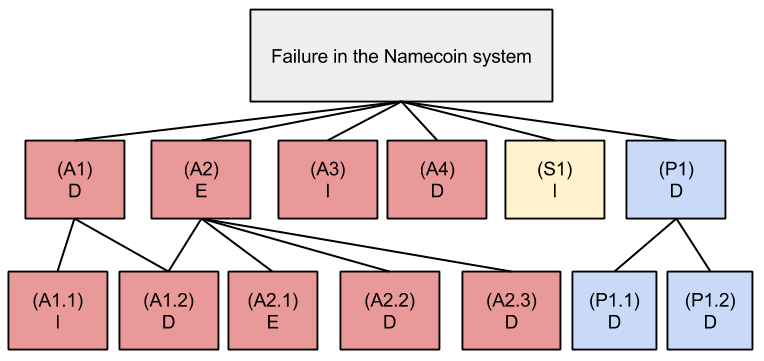
\includegraphics[width=90mm]{Pics/smallattacktree.png}
    \caption{Representation of the attack tree risk analysis.}
    \label{fig:smallattacktree}
\end{figure}

\subsection{Attacks}
\textbf{(A1) Build a fork of the block chain.}
The first attack possibility (A1) is to build a fork of the block chain. As long as this separate branch is smaller than the main branch, it does not affect the rest of the network since the network nodes always chooses the branch which is the longest. \\\\
\noindent
\textbf{(A1.1) Acquiring more than $\boldsymbol{50 \, \%}$ of the hash rate.} If the attacker has more than $50 \, \%$ of the hash rate\footnote{Hash rate is the rate of the number of hashes you can calculate per second.}, the attacker can alter transaction information in the most recent block. This allows the attacker to send a transaction to another user and then remove the transaction from the block which it is stored in, causing the attacker to regain her amount of Namecoins which she sent. This node's value is set to $I$ due to the fact that the interest of mining coins has increased greatly in the recent years and it would take a vast amount of resources to acquire more than $50 \, \%$ of all the hash rate in the network. As of May 2014 the network hash rate is $52.289 \; Phash/s$, which can be seen in Figure~\ref{fig:hashrate}.  We illustrate how much this is through the following example; if you want to buy a device that is developed purely for mining, one of the fastest is the Extolabs EX1. The EX1 gives you $3.6 \; Thash/s$ for the price of \$9499. This means you need approximately \$57 million dollar to acquire half the hash rate of the network \cite{extolabs}. \\\\
\noindent
\textbf{(A1.2) Brute force attack.} Another possible attack, which is similar to the previous attack, is the brute force attack (A1.2). For this attack to have a reasonable probability, it is required for the attacker to possess a large amount of the hash rate available (most likely more than $50 \, \%$) or else it would require an enormous amount of luck in order to be achieved. The attacker first transmits a transaction to the merchant to pay for the product, while mining a block chain privately, i.e. without broadcasting to the network. In this alternative block chain, a double-spending transaction is included instead of the legitimate one which was sent to the merchant. The merchant then waits for $n$ confirmations\footnote{A confirmation of a transaction is when a block is added and linked to the block which contains the transaction.}, before sending the product ordered by the attacker. If the attacker happened to successfully mine more than $n$ blocks at this point in time, she releases and broadcasts her local fork and regains her coins. And if the attacker has not achieved $n$ blocks, she can continue extend her fork with the goal of catching up with the network main branch. If the attacker's attempts to compete with the network branch fails, the payment of the product will go through to the merchant and the attack has failed. As mentioned earlier, the probability of success for this attack is a function of the attackers hash rate (as a proportion in percent of the total network hash rate) and the number of confirmations which the merchant awaits before approving the transaction \cite{hashratespending}. \\\\
The level of difficulty for this attack is set to $D$, based on the fact that the probability of success depends on the attackers amount of hash rate, i.e. if the attacker has enough hash rate, the attack is not improbable to execute.

\pagebreak

\noindent
\textbf{(A2) Double spending attack.}
The second attack possibility is to perform double spending, which can be simply be explained as to spend the same Namecoins more than once. As Figure~\ref{fig:smallattacktree} illustrates there are four possible ways to accomplish this:\\\\
\noindent
\textbf{(A2.1) Race attack.} The race attack consists of an attacker sending two conflicting transactions, i.e. transactions consisting of the same Namecoins, to a merchant and into the network. Due to the fact that there are thousands of Namecoin clients constantly searching, increases the probability that it will be recognized by the network and inserted into a block, before the merchant finds it. This results in the case where the merchant has sold a product without receiving a payment. Merchants who accept payments on seeing \emph{unconfirmed}-status on the transactions are especially vulnerable to this attack. \\\\ The level of difficulty for this attack is set to $E$ due to the fact that it does not require any vast amount of resources to perform \cite{bitcoin-attacks}. \\

\noindent    
\textbf{(A2.2) Finney attack.} The Finney attack is when an attacker mines a block privately containing a transaction from the attacker to herself.  The attacker then buys a product from a merchant using the same coins which was included in the private block. Before the transaction to the merchant is included in a new block, the attacker broadcasts her block, containing her transaction to herself.\\\\
\noindent
If this is successful the attack is successful, because the coins in the transaction to the merchant is now spent elsewhere, that transaction will become invalid and no coins will be spent. If another client broadcasts her block before the attacker, her private block will no longer be valid and she will have to mine another block and begin a new attempt of the attack. If the attack is successful, the attacker gains the product, the block reward and she retains her coins. If someone else broadcasts a block before the attacker she will lose both the block reward and her coins \cite{bitcoin-attacks}. \\\\
The node value for the Finney attack is set to $D$, based on the fact that the attacker has to convince the merchant that the transaction is legitimate and that if another client mines a block before the attacker has broadcasted his, the attack has failed. \\

\noindent
\textbf{(A2.3) Vector76 attack.} The Vector76 attack is a combination of the previous explained Race attack and Finney attack, where the attacker double spends Namecoins using a transaction which has been confirmed once.\\\\
\noindent
The attack is accomplished as follows; initially the attacker establishes a direct connection to the target, by monitoring for which nodes are the earliest to broadcast transactions from the target. The next step for the attacker is to start mining for a block and create a transaction with a large deposit to the target. Neither the mining of the block nor the transaction are broadcasted. When the mining is successful and a block $A$ is created, the attacker awaits for another miner to succeed with the creation of a block $B$. When the other miner creates $B$, the attacker immediately broadcasts $A$ to the target.

\pagebreak

\noindent
If the target notices the attackers block $A$ before block $B$ it will be accepted. This will make the target believe that the attackers transaction (which was in the attackers block $A$, mined privately) is valid and in the block chain. The block chain is now forked and the target of the attack will be under the impression that $A$ is the legitimate one, while the rest of the network will believe that the other block, $B$, is the real one. The attacker then requests a withdrawal and the target creates a transaction and sends the large amount of coins to an address under the control of the attacker. The network part that did not receive $A$ will accept this transaction and vote to include it in the next block. This means that the withdrawal will be a part of the main branch of the block chain while the deposit will not \cite{bitcoin-attacks}. \\\\
In order for the attack to be successful, the miners in the network that saw block $B$ first has to exceed the number of miners that saw block $A$ first and thus continued mining for that block to be included in the block chain. If the attack is executed without any problems, the attacker loses the reward for finding a block but gains the coins spent by the target. If the attack is unsuccessful the attacker loses the deposit made to the target, but at least gains the block reward from mining. \\\\
The level of difficulty for the Vector76 attack is set to $D$. This value was set due to the fact that timing is a major factor which needs to be precise in order for the attack to be successful, along with the property that the majority of the miners has receive the real block first, and not the attackers block. \\\\
\noindent
\textbf{(A3) Break the cryptographic hash function (SHA-256).} The attack which involves breaking the hash function is based on the possibility of someone figuring out how a hash is calculated with SHA-256. Breaking this hash function has the consequences of allowing the attacker to mine all blocks and therefore make changes to the block chain as she like. Because of the design of a hash function this is supposedly very hard to do. There is however several broken hash functions e.g. MD5, which was believed to be unbreakable for a long time, but eventually it was cracked. \\\\
The difficulty of this attack is set to $I$ because there is no known attacks to it and as far as we know no one is close to cracking it. \\

\noindent
\textbf{(A4) Sybil attack.} The Sybil attack is an attack that tries to isolate an attacked user from the rest of the peer-to-peer network to control what data they get and do not get. The attacker has to control a lot of nodes and use these as "fake"-nodes. The attacker connects all of these nodes to the network. Then the attacker will try to find a user that is only connected to her fake nodes. She will then stop the nodes from broadcasting found blocks to this user and therefore isolate her from the rest of the network. Since the user is now isolated in a subnet controlled by the attacker she can easily conduct for example double spending attacks onto the user.\\\\
We classified this attack as a $D$ because it is possible, but it requires a lot of resources from the attacker. The easiest way to realize you are being attacked is to check for irregular changes in the network hash rate. When you get isolated it will always drop to a very low number compared to what it usually is \cite{bitcoin-attacks}.
\noindent
\subsection{System flaws} Our first and only system flaw, (S1), is that all the Namecoins are destroyed. There is only 21 million NMC and every time someone registers a domain name 0.01 NMC is destroyed. If 2.1 billion domains are registered there will actually be no more Namecoins to spend. We decided to put this risk as $I$ because there is only about 1 billion domains registered on the Internet today and the Namecoin creators have also stated that the transaction fee of 0.01 NMC is not final and can be changed if this becomes a problem \cite{Namecoin}.

\subsection{Psychological attacks}
There are also psychological attacks that can compromise Namecoin. For the system to work there has to exist a lot of honest miners who are not trying to attack the system. If someone can hurt the Namecoin image, (P1.1) and make people distrust the system many honest miners will leave. When this happens the system becomes vulnerable to all sorts of attacks, because of its peer-to-peer structure. \\\\
The system is also built upon a hash function (SHA-256) and if someone claimed to have broken this, (P1.2), it could cause a lot of distrust in the system. If the miners do not trust the system they will stop mining and the system will fall apart. We decided to label both psychological attacks as $D$ because it is not easy to make people stop trusting a system without real proof, which is very hard to get \cite{bitcoin-attacks}.

\section{Discussion}
In this section we will discuss our risk analysis and also compare our results to current solutions.

\subsection{Risk analysis}
The double spending attacks; the Finney attack, the Vector76 attack and the Race attack, are mitigated through use of confirmations. If all users wait for the recommended amount of confirmations on their transactions, these attacks will not be successful. The brute force attack is not likely to succeed unless you have more than $50 \, \%$ of the hash rate in the network. As mentioned earlier this is not a attack with much reward, since it takes a lot of resources to perform and it is not certain that it will reward the attacker enough. The Sybil attack requires a lot of resources and it has very small, if any, rewards for the attacker. It is also easy to recognize if you are being attacked even with small insight into how the system operates. The last attack marked with $D$ is to demotivate miners, through either creating distrust in the system or the hash function. This can be countered through PR-marketing by trustworthy people describing how the system works and why it is safe. The rest of the attacks are marked as $I$ and are therefore so improbable that they do not need precautions.\\\\
Namecoin is a new sort of system built on the block chain from 2008. Today it is not used for authentication, but for domain name registering only. In version 2.0 it is planned to include support for TLS fingerprints which will replace certificates. 

\pagebreak

\noindent
If you buy a domain name you can also register a public key with this domain and save this in the block chain. Because of the structure of the block chain it is only possible for you to change this key, but everyone can see it and the changes made to it. Whenever someone wants to communicate with your domain they will look for it in the block chain and will also find the TLS fingerprint. This way you get both the right IP-address but also a secure way to connect to an authenticated client.\\\\ As we can see in the risk analysis the only attacks that can really hurt the system is if someone can get more than $50 \, \%$ of the hash rate, either through massive collection or through demotivating other miners. If someone can do this they will be able to rebuild the block chain after their own taste and the system does not work as intended. Although, we find this highly unlikely to occur due to the extreme amount of hash rate needed. If someone spends \$57 million on equipment that can only be used for mining she will be reluctant to abuse the system. If people do not use it anymore she has \$57 million worth of equipment with little use. This results in the fact that a user will profit more on following the rules, rather than abusing the system. 

\subsection{Comparison to current authentication mechanisms}
The biggest difference between Namecoin, CAs and Web of trust is the network structure. In the CA solution it is an infrastructure-based network where you trust several centralized authorities. In the Web of trust and Namecoin solutions you depend on a peer-to-peer network with decentralized trust.\\\\
Both Web of trust and the CA solution needs total confidence in every trusted node or CA. If one node or CA becomes malicious the entire system is compromised and you can no longer trust it. If you use Namecoin, more than $50 \, \%$ of the networks hash rate needs to become malicious before the system is compromised. Because of the massive amount of hash rate in the network it is not likely that this will occur. In our risk analysis we did not find any attacks with dire consequences which have not been prevented. Because of this we can replace the current authentication system with Namecoin and end up with a more secure system. Namecoin works like an online bulletin board which can only be changed through majority decisions. Because of this structure we can store authentication information on this board and be certain that this is correct information. With this system you do not need to trust every single node in the network, but you must trust a majority of the users. Therefore we have found it to be the better solution for the problem of authentication.
    
% SKA TA UPP ETISKA OCH SAMHÄLLELIGA ASPEKTER AV ARBETET. SE MALL FÖR FLER INFO
\subsection{A broader perspective}
In the modern society a lot of sensitive information, for example bank transactions, are sent over public networks and this has to be secure. Public-key encryption is widely used to ensure secure communication with no eavesdropping. Authentication is needed to verify the identity of the recipient, so that you can be certain that your information is sent to the intended entity.

\pagebreak

\noindent
If we can not use proper authentication we can never be certain that our information is not compromised. Because of the extensive use of the Internet today, combined with the increasing usage in the future, security on the Internet becomes more important every day. In our work we discovered that the currently used authentication systems are flawed and this is a threat against security on the Internet. If these systems are not replaced or fixed, a lot of traffic will be considered secure by the communicating entities, but could in fact be compromised.  

\section{Conclusions}
In this report we have highlighted some of the existing schemes for public-private key encryption and explored their security issues. We have found that although currently used schemes are still mathematically safe, issues arise in implementation. Specifically, authentication of public keys is still an issue that threatens currently used public-private schemes.\\\\
We have analysed an alternative solution to the issue of authentication. Our suggestion is to replace the current solution, CA, with the Namecoin system which can be used for both DNS and authentication. One of the major advantages with Namecoin, compared to the use of certificate authorities, is that the system does not fail if one trusted entity becomes malicious. The biggest risks we found were if someone controlled more than $50 \, \%$ of the hash rate in the network or if someone broke the SHA-256 hash function. Both of these risks are improbable and therefore the system can be considered safe. All of these will be implemented in the version "Domain names v2.0" and be available when it launches. 

%-------------------------------------------------------------
%   END OF DOCUMENT
%-------------------------------------------------------------
\bibliographystyle{ieeetr}
\bibliography{sigproc}  % sigproc.bib is the name of the Bibliography in this case
% You must have a proper ".bib" file
%  and remember to run:
% latex bibtex latex latex
% to resolve all references
%\balancecolumns

\appendix
\chapter{Figures}
\chaptermark{}
\begin{figure}[h!]      %   PIC: ATTACK TREE 
    \centering
    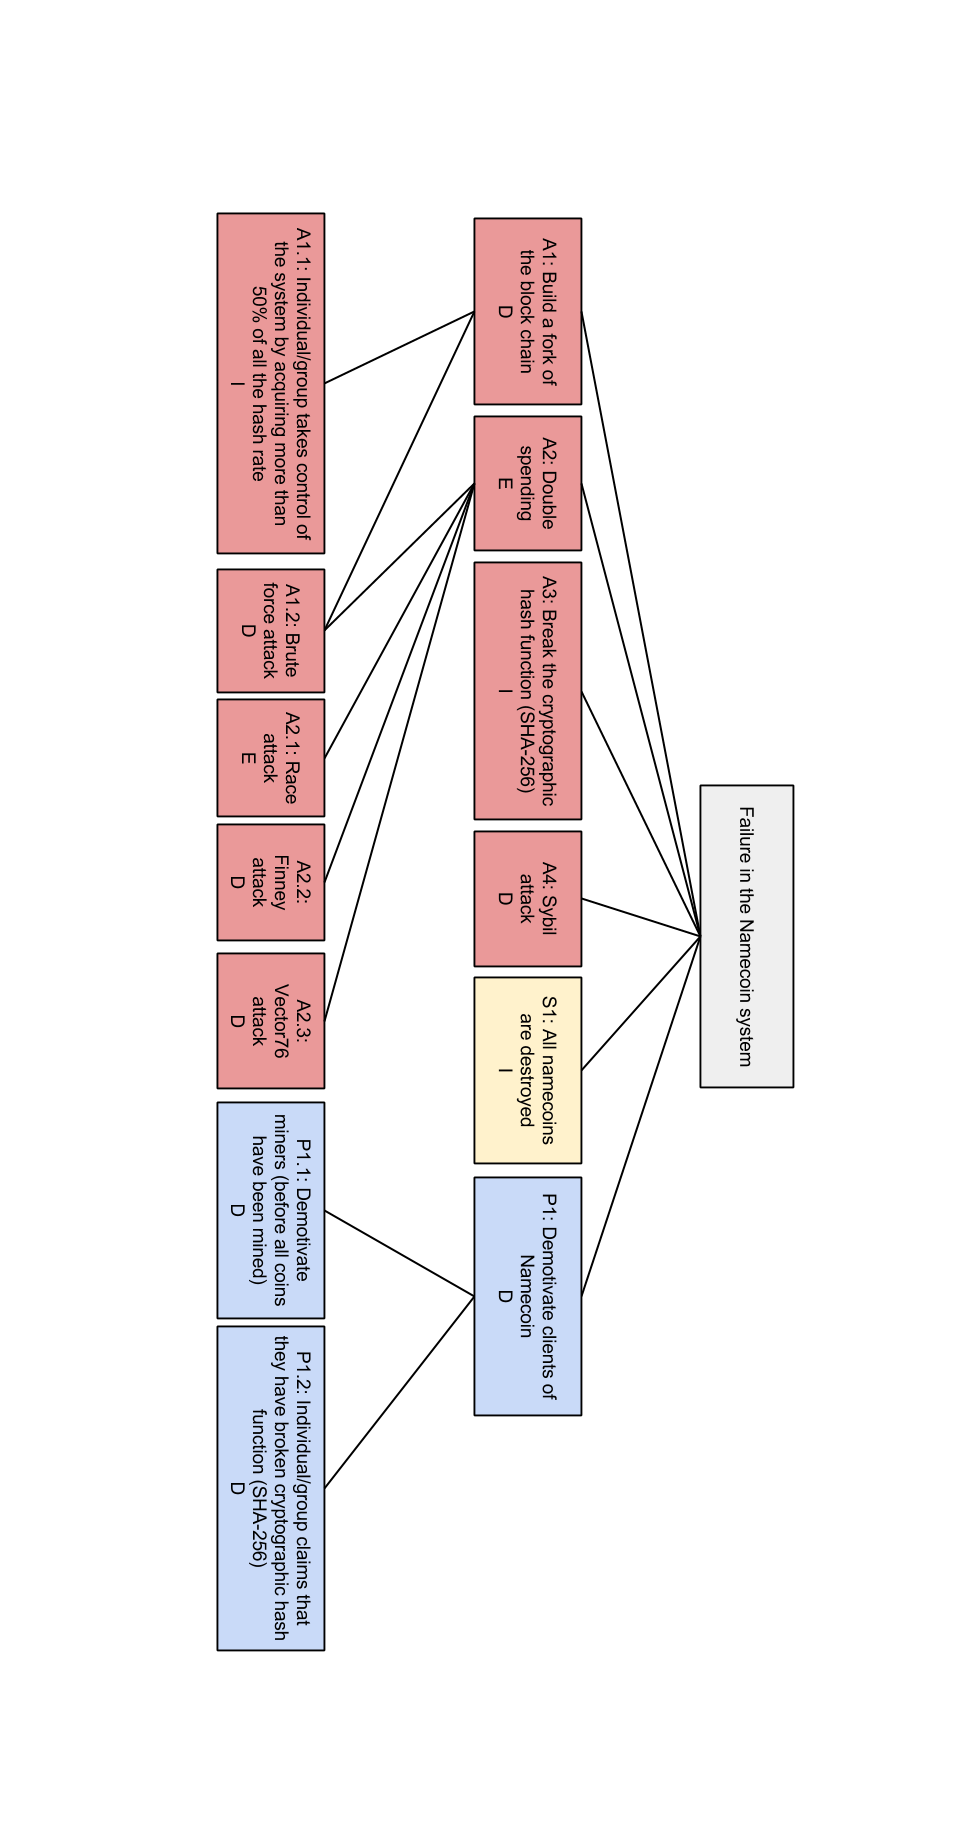
\includegraphics[width = 120mm, height = 155mm]{Pics/attacktree.png}
    \caption{The attack tree generated from our risk analysis. }
    \label{fig:attacktree}
\end{figure}

\begin{figure}[h!]      %   PIC: Hash rate 
    \centering
    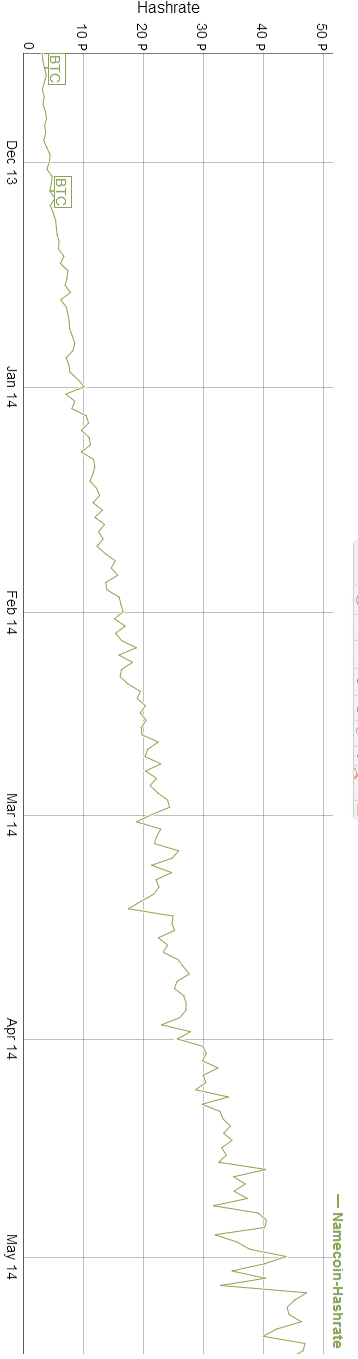
\includegraphics[height = 155mm]{Pics/hashrate.png}
    \caption{The hash rate of the Namecoin network the last 6 months. Measured in $hash/s$. Available at: http://bitinfocharts.com/comparison/hashrate-nmc.html}
    \label{fig:hashrate}
\end{figure}

\end{document}
